\documentclass[11pt,a4paper]{article}
\usepackage{acl2015}
\usepackage{times}
\usepackage{url}
\usepackage{latexsym}
\usepackage{lipsum}
\usepackage{natbib}
\usepackage[font=small, labelfont=bf]{caption}
\usepackage{amsmath}
\usepackage{graphicx}
\usepackage[hidelinks]{hyperref}

\title{Report: Dialog Act Classification\\\textit{using Word Embeddings \& Acoustic Features}}

\author{Jens Beck \\
  {\tt jens.beckl@ims} \\\And
  Fabian Fey \\
  {\tt fabian.fey@ims} \\\And
  Richard Kollotzek \\
  {\tt richard.kollotzek@ims} \\}

\date{}

\begin{document}
\maketitle

\begin{abstract}
\lipsum[2-2]
\end{abstract}

\section{Introduction}
The general task is to classify lexical and auditory speech into one of four predefined \textit{dialog act classes}. A \textit{dialog act}, in this context, represents informal information of how a dialog system should respond to a users input. The four provided classes are \textit{statement, opinion, question} and \textit{backchannel}. To solve this task we developed \textit{convolutional neural networks} (CNN) that use lexical and acoustic features. For the development and training of the systems a subset of the \textit{Switchboard Dialog Act Corpus} was used. In next chapters we discuss the development of the systems and subsequently to that the research question \textbf{INSERT HERE}.

\section{Data \& Data Preperation}
In this section we discuss the \textit{Switchboard Dialog Act Corpus} and the extraction of the lexical and acoustic features.

	\subsection{The Switchboard Dialog Act Corpus}
	The \textit{Switchboard Dialog Act Corpus} \cite{switchboard}, from now on abbreviated as \textit{SwDA}, consists of recordings with corresponding transcripts. Each of these recordings is assigned to one of 42 \textit{dialog act classes}. For this project we reduced the amount of classes down to four which are \textit{statement, opinion, question} and \textit{backchannel}. These classes are supersets of the 42 \textit{dialog act classes} defined in the \textit{SwDA}. The distribution of the four classes within the training, development and test set are shown in Table \ref{tab:dataDistribution}.
	%todo Examples for the four classes if more text is needed
	\begin{table}[]
		%todo Own tabel design
		\centering
		\begin{tabular}{ r | c c c }
			& \textbf{training} & \textbf{dev} & \textbf{test} \\
			\hline
			opinion ($\sim$17\%) & 4984 & 1068 & 1070 \\
			question ($\sim$8\%) & 2150 & 460 & 463 \\
			backchannel ($\sim$24\%) & 6792 & 1455 & 1458  \\
			statement ($\sim$51\%) & 14459 & 3098 &  3099  \\
			\hline
			sum & 28385 & 6081 & 6090 \\
		\end{tabular}
		\caption{Displays the distribution of the four classes in the three data sets.}
		\label{tab:dataDistribution}
	\end{table}	
	The numbers illustrate a huge imbalance between the \textit{statement} class and the other three classes. However, we decided against reducing the data into equally distributed sets because this would exclude at least one third of the training data. This is important to keep in mind for the evaluation of the systems because an educated guess would have an accuracy of around 51\% by assigning all test examples to the \textit{statement} class.

	\subsection{Input Data Generation}
	Lexical and acoustic features were employed in our systems and had to be extracted and formatted into a machine readable format. For the lexical features we decided to use \textit{Google's} freely accessible word embeddings which were trained on 100 billion words \cite{word2vec}. As for the acoustic features we relied on \textit{Mel Frequency Cepstral Coefficient} (MFCC) features which were extracted with the \textit{openSMILE} feature extraction tool \cite{opensmile}. To ensure that data of different utterances could not be mixed the lexical and acoustic inputs were always stored with their respective one-hot vector in a triple data structure.
	
	\subsubsection*{Lexical Features}
	\label{sec:lexicalFeatures}
	The word embedding matrix $E$ was generated by assigning each word to its corresponding 300 dimensional vector of the \textit{Google word2vec} model. If a word was not included in the model it was assigned a randomly generated 300 dimensional vector. Furthermore, we introduced a padding vector for the case that a sentence was shorter than our maximum sentence length. We decided to restrict the length of a single utterance to 100 words to not exclude to much lexical features for long utterances. The final size of the embedding matrix $E$ was $11825  \times 300$.
	\begin{center}
		$ E= 
		\begin{bmatrix}
		v_{1,1}	&  \dots	 & v_{1,300}    \\
		v_{2,1}	 	& \dots  & v_{2,300} 	\\
		\vdots	 	& \ddots & \vdots		\\
		v_{i,1} 	& \dots	 & v_{i,300}
		\end{bmatrix}
		$
	\end{center}
	\vspace{0.3cm}
	The lexical input for our systems is a vector $x_{lex}$ were each word is represented by the index $i$ of its corresponding vector in the embedding matrix $E$. The vector $x_{lex}$ has a length of 100. Each element represents the index of a word in the utterance. The vector $x_{lex}$ has the following shape: $x_{lex} = [i_{1}, i_{2}, ..., i_{100}]$ where $i$ represents the index.
	
	\subsubsection*{Acoustic Features}
	Each utterance had its acoustic features formatted into a matrix $X_{aco}$ of shape $13 \times 2000$. This matrix was generated by arranging 2000 \textit{MFCC-frames} into a matrix. Each \textit{frame} hereby consisted of 13 coefficients. The chosen \textit{frames} were the first and last thousand \textit{frames} of the audio recording. If a recording had less than 2000 \textit{MFCC-frames} the matrix was padded with zero vectors.
	
	\begin{center}
		$ X_{aco}= 
		\begin{bmatrix}
		a_{1,1}	&  \dots	 & a_{1,2000}   \\
		a_{2,1}	 	& \dots  & a_{2,2000} 	\\
		\vdots	 	& \ddots & \vdots		\\
		a_{13,1} 	& \dots	 & a_{13,2000}
		\end{bmatrix}
		$
	\end{center}
	\vspace{0.02cm}
	
	\noindent Afterwards, to use minibatch processing it was necessary to reformat $X_{aco}$ into a vector $x_{aco}$ with the shape $1 \times 26000$.
	
%	\subsubsection*{Minibatch processing}
%	batchList = [ (1Batch-Features, 1Batch-MFCC, 1Batch-Labels), (2Batch-Features, 2Batch-MFCC, 2Batch-Labels), ...]
	
\section{Baseline Systems}
The architecture of the proposed \textit{AcoLex} system is depicted in Figure \ref{pic:sysArchitecture}. In this section we will explain the complete architecture of the system. Furthermore, we will discuss its two core components: the lexical and the acoustic model.

\begin{figure}[h]
	\centering
	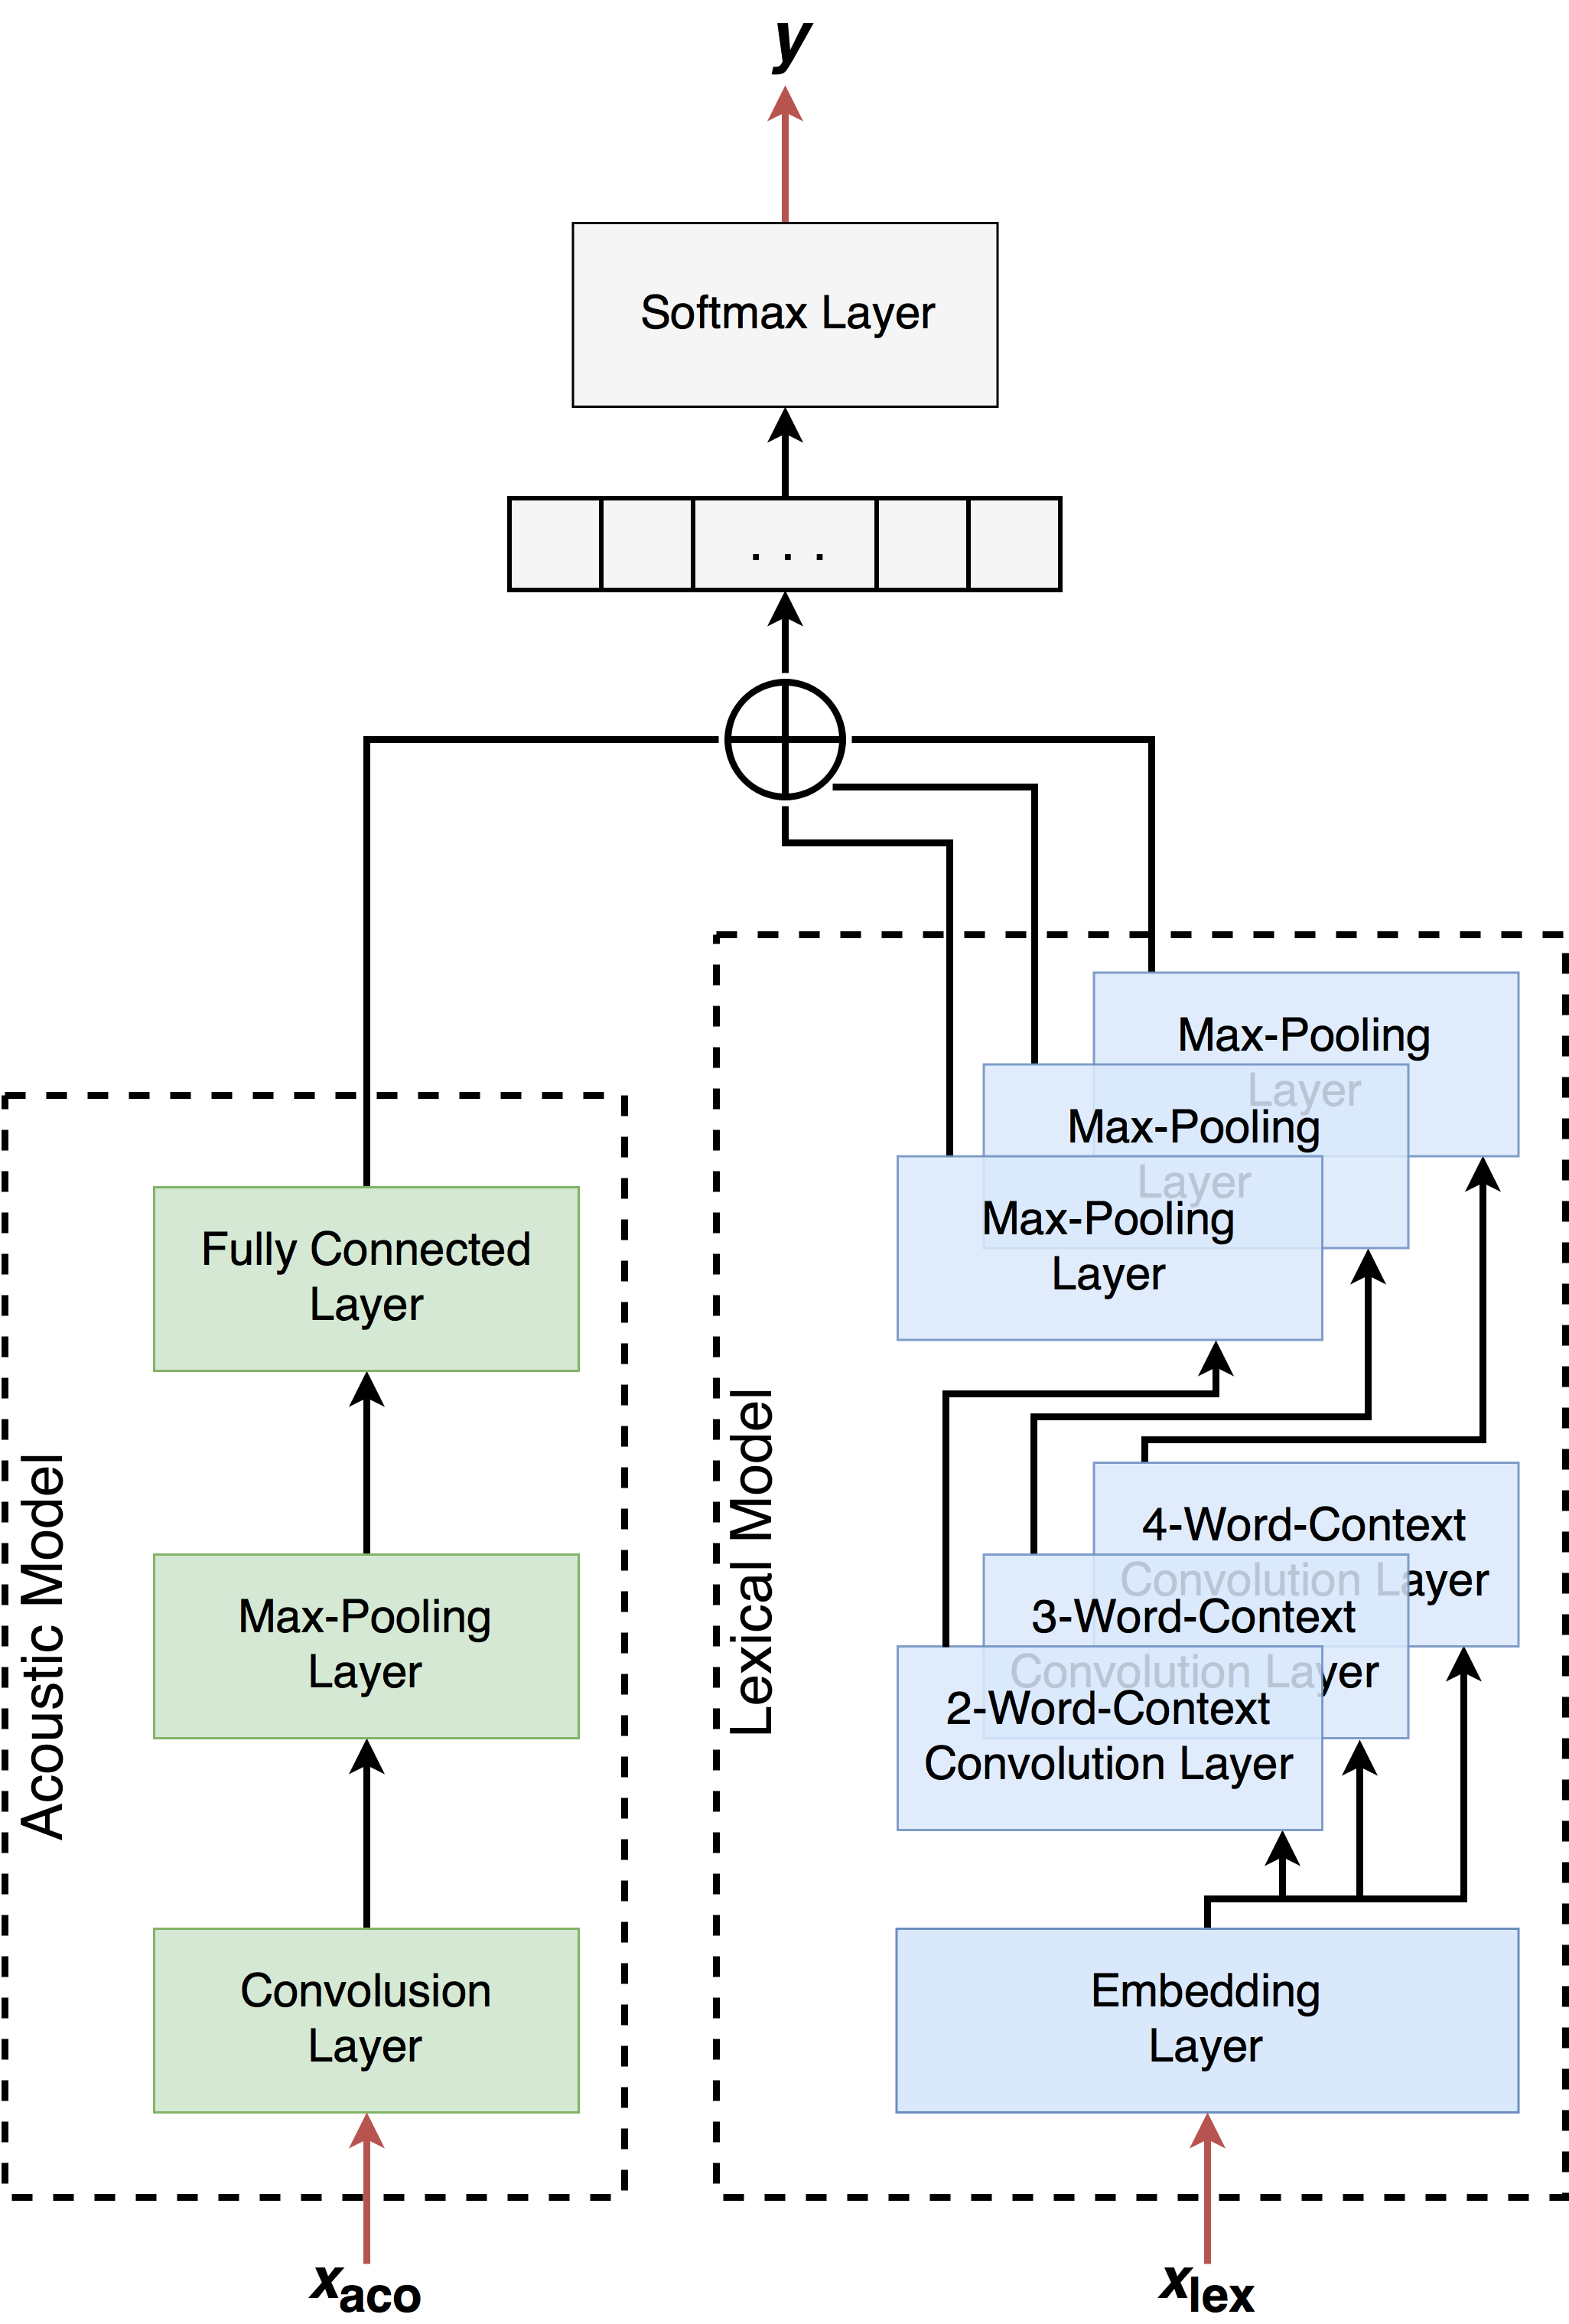
\includegraphics[width=1\linewidth]{Bilder/acolex_CNN_paper.png}
	\caption{bla bla bla}
	\label{pic:sysArchitecture}
	%todo Bild verbessern, maxpooling bei LM hinzufügen, Bildunterschrift hinzufügen
\end{figure}

\subsection{Lexical Model}
The \textit{lexical model} (\textit{LM}), depicted on the right side in Figure \ref{pic:sysArchitecture}, consists of three layers. The architecture is based on the system introduced by Kim (2014) \cite{Kim_2014}. The first layer is an \textit{embedding layer} which was initialized with the \textit{embedding matrix} $E$ described in Section \ref{sec:lexicalFeatures}. The benefits of using an embedding layer is a significant reduction of the time needed to import the input files due to storing the vector of each word only once. Furthermore it enables the tuning of the \textit{embedding vectors} for the classification task. The second layer is a \textit{convolution layer} which uses three different filter sizes to capture different word contexts, namely \textit{2-word-}, \textit{3-word-} and \textit{4-word-contexts}. Overall 300 filters are applied in the LM, were each filter type is used 100 times. The last layer is a \textit{max-pooling layer} that returns the highest value of each filter output. Therefore, the final output of the LM are three 100 element long vectors.

\subsection{Acoustic Model}
%todo cite Ortega 
The \textit{acoustic model} (\textit{AM}), shown on the left side in Figure \ref{pic:sysArchitecture}, is developed similarly to the acoustic model presented by Ortega et. al (2018) \cite{OrtegaVu_2018}. Like the \textit{LM} it utilizes three different layers. The first layer is a \textit{convolution layer} with one filter type that captures 100 \textit{MFCC-frames} at a time. We decided to use a stride of 50 to significantly reduce the processing time. The second layer is a \textit{max-pooling layer} similar to the one in the \textit{LM}. This layer returns a 100 element long vector. This output is fed into a \textit{fully connected layer} which returns the final output of the \textit{AM} which is a 100 element long vector.

\subsection{AcoLex Model}
Our proposed \textit{AcoLex Model} employs a \textit{bi-CNN} that consists of the \textit{LM} and the \textit{AM} to simultaneously process lexical and acoustic features. The outputs are then concatenated into one 400 element long vector which is then passed into a \textit{softmax layer} to perform the \textit{dialog act classification task}. The final output is a four element long vector were each element represents the probability for one \textit{dialog act class}.

\section{Training}
The system was trained for 21 epochs with the \textit{stochastic gradient descent} optimization algorithm over mini-batches of size 100. The learning rate was fixed to 0.01. The tunable hyperparameters are shown in Table \ref{tab:hyperparameters}.

\begin{table}[h]
	%todo Own tabel design
	\centering
	\begin{tabular}{ l | c | c}
		\textbf{Hyperparameter} & \textbf{LM} & \textbf{AM} \\
		\hline
		Filter width & 2, 3, 4 & 100 \\
		Activation function & Relu & TanH \\
		Word embeddings & word2vec & -- \\
		MFCC features & -- & 13 \\
		Dropout$^\ast$ & 0.5 & 0.5 \\
		Learning Rate$^\ast$ & 0.01 & 0.01 \\
		Mini-batch size$^\ast$ & 100 & 100 \\
		\# Feature maps$^\ast$ & 100 & 100 \\
	\end{tabular}
	\caption{Hyperparameters marked with $^\ast$ are model independent and were set for the whole system.}
	\label{tab:hyperparameters}
\end{table}	

\section{Results}

\begin{table}[h]
	%todo Own tabel design
	\centering
	\begin{tabular}{ l | c c}
		\textbf{Model} & Dev Accuracy & Test Accuracy\\
		\hline
		Acoustic & &  \\
		Lexical & 77.52 & 77.40 \\
		AcoLex & 80.24 & 79.93 \\

	\end{tabular}
	\caption{Hyperparameters marked with $^\ast$ are model independent and were set for the whole system.}
	\label{tab:results}
\end{table}	

\section{Research Question: None}

\section{Conclusion}

\bibliographystyle{abbrv}
\bibliography{bibliography}
\nocite{*}
%todo Own cite style

\end{document}

